\section{5.1 Purpose and status}\label{purpose-and-status}

MGP-6 v2 is an \textbf{author-designed 180-scenario diagnostic slice},
not an independent community benchmark; every claim in this thesis
phrases it as such. Its purpose is to isolate write-time governance
competence --- when to keep, when to supersede, when to abstain ---
under controlled conflict structure, so that decision failures are
attributable and countable. Verified against the raw JSONL on 2026-07-12
(\texttt{benchmarks/mgp6/data/mgp6\_v2.jsonl}).

\section{5.2 Composition}\label{composition}

{\def\LTcaptype{none} % do not increment counter
\begin{longtable}[]{@{}
  >{\raggedright\arraybackslash}p{(\linewidth - 2\tabcolsep) * \real{0.5000}}
  >{\raggedright\arraybackslash}p{(\linewidth - 2\tabcolsep) * \real{0.5000}}@{}}
\toprule\noalign{}
\begin{minipage}[b]{\linewidth}\raggedright
Property
\end{minipage} & \begin{minipage}[b]{\linewidth}\raggedright
Value
\end{minipage} \\
\midrule\noalign{}
\endhead
\bottomrule\noalign{}
\endlastfoot
Scenarios & 180 \\
Conflict types & T1--T6, 30 each (type definitions:
\texttt{benchmarks/mgp6/mgp6\_v2\_spec.md}; T3 = implicit conflict) \\
Gold actions & SUPERSEDE 90, ABSTAIN 66, KEEP 24 \\
Splits & train 60 / dev 30 / test 90 \\
Query modes & direct\_recall 108, premise\_resistance 45,
implicit\_application 27 \\
\end{longtable}
}

The gold-action distribution is author-imposed rather than
population-derived. SUPERSEDE is the majority class (90/180), while
ABSTAIN and KEEP account for 66 and 24 items. Macro-F1 therefore
accompanies accuracy, but neither metric repairs the more serious
shortcut defect: conflict type deterministically identifies the action
in this pilot. The distribution must not be interpreted as an estimate
of deployment prevalence.

\section{5.3 Unit of analysis and split
policy}\label{unit-of-analysis-and-split-policy}

Each scenario has a stable \texttt{scenario\_id}, an interaction context
establishing prior memory, a candidate event, a gold action, a conflict
type, a split, and a query mode for the downstream probe. Evaluation
joins by stable ID. The rule controller was developed against train/dev;
therefore the \textbf{test-split figures (n=90) are always reported
first} and full-corpus figures second (§7.2), a split-hygiene rule
enforced by the claims matrix.

\section{5.4 Query modes: probing the state, not just the
decision}\label{query-modes-probing-the-state-not-just-the-decision}

Each scenario carries a downstream probe in one of three modes:
\textbf{direct recall} (does the current value surface?),
\textbf{premise resistance} (the probe asserts a stale or false premise;
a governed system must resist it), and \textbf{implicit application}
(the current value must be used without being named). These modes
connect decision correctness to memory-state behavior; premise
resistance in particular is where the rule and LLM controllers diverge
most sharply (1.0 vs 0.0889, §7.2). The construct is adjacent to STALE's
read-side premise-resistance probing \citep{chao2026stale}; MGP-6 v2
differs in scoring the \emph{write actions} that produce the probed
state.

\section{5.5 Annotation evidence --- stated
precisely}\label{annotation-evidence-stated-precisely}

Two distinct components, never to be conflated (source of truth §1.2):

\begin{enumerate}
\def\labelenumi{\arabic{enumi}.}
\tightlist
\item
  \textbf{One independent annotator} covered the 90-item test split
  (\texttt{benchmarks/mgp6/annotations/human/}): raw agreement
  \textbf{0.9889} {[}0.9667, 1.0{]}, \textbf{Cohen's κ 0.98146}
  {[}0.93997, 1.0{]}, macro-F1 0.9913, exactly \textbf{one disagreement}
  --- \texttt{MGP6V2-T3-TEST-016} (implicit conflict; annotator ABSTAIN
  vs gold SUPERSEDE). Caveats: n = 1 annotator; the annotator's
  independence and human identity rest on author attestation; this is
  \textbf{not} multi-human inter-annotator agreement.
\item
  \textbf{A four-LLM audit panel} (geminiPro, gptSolHigh, kimi, z) over
  the same 90 items: \textbf{Fleiss κ 0.9815}, unanimous on 88/90,
  per-model agreement with gold 1.0 / 0.9778 / 1.0 / 1.0, majority vote
  \textbf{100\%} versus gold. This is a model audit, not human IAA.
\end{enumerate}

Additional disclosures: the human review sheet exists but is 0/180
filled; dataset documentation dated 2026-07-10 predates both annotation
sets (2026-07-11) and wrongly states agreement was unmeasured ---
reconciled in this thesis and flagged for the release. The single
disagreement is retained as an adjudication item and used for
sensitivity discussion (§8.4), not silently relabeled. Because the
labeling manual was authored alongside the scenarios, the panel may
share the author's reading; this construct-validity limit is threat C2
in Chapter 9.

\begin{figure}
\centering
\pandocbounded{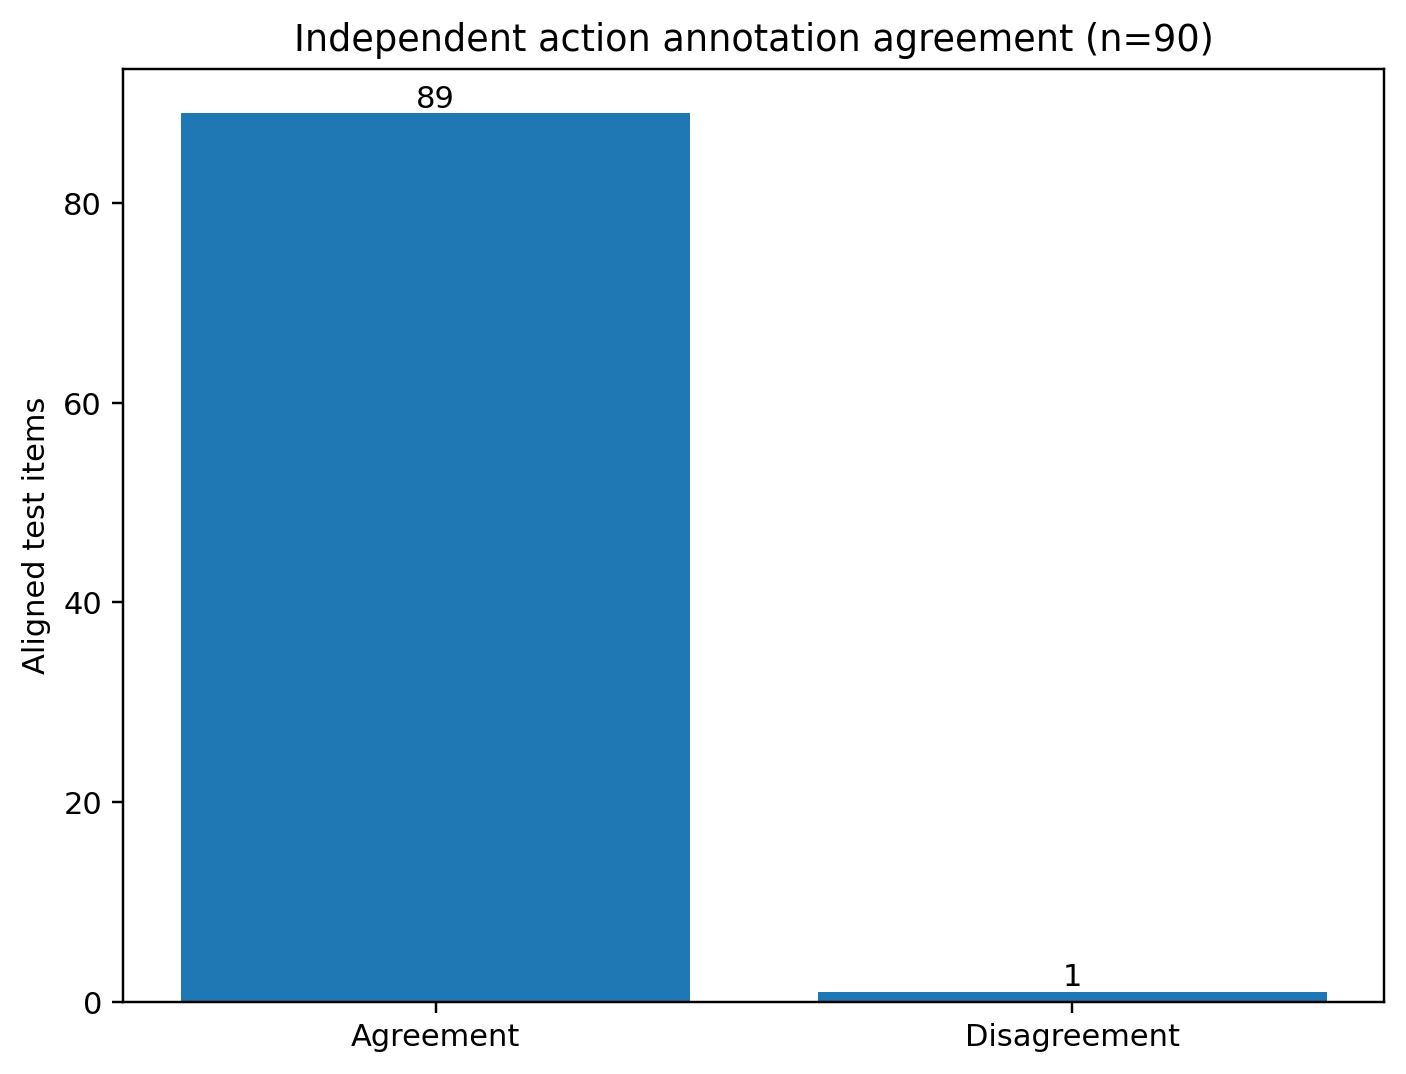
\includegraphics[keepaspectratio]{../../docs/figures/figure_04_annotation_agreement.png}}
\caption{Annotation agreement.}
\end{figure}

\section{5.6 Baselines embedded in the
instrument}\label{baselines-embedded-in-the-instrument}

Four reference systems establish what the slice measures: B1 no-memory,
B2 flat retrieval, B3 recency preference, B4 naive overwrite. B2--B4
cannot express abstention (invalid-commit rate 1.0 by construction on
gold-ABSTAIN items), which is precisely the governance gap the
instrument is designed to expose; consequently their comparisons with
the controller are diagnostic, not general-capability results (§7.4,
threat S3).

\section{5.7 Relationship to
LongMemEval-M}\label{relationship-to-longmemeval-m}

The stratified LME-M slice (180 items, 6 competencies × 30, seed 0,
built deterministically by \texttt{scripts/build\_stratified\_slice.py};
the underlying LongMemEval data is external and not redistributed)
addresses the downstream layer: whether governed memory supports later
answers over long histories \citep{wu2025longmemeval}. A system can
occupy any cell of the decision-correct × answer-correct table. Chapter
7 uses the archived downstream runs only as failure analysis because
provider contamination, replay selection, and incomplete coverage
prevent a clean estimate of cross-layer association.

\section{5.8 Known metric issues (disclosed, excluded from
claims)}\label{known-metric-issues-disclosed-excluded-from-claims}

As shipped, \texttt{over\_forgetting\_rate} and
\texttt{under\_forgetting\_rate} saturate at 1.0 for every system and
are uninformative; they appear in no claim in this thesis (ledger
\texttt{known\_metric\_issues}). The \texttt{invalid\_commit} metric was
revised during the project; all reported numbers use the revised
definition, and pre-revision \texttt{.bak} files are preserved (threat
I6).
